%  ----------------------------------------------------------------------------
%
%       Copyright (for the thesis) 2009 by [author - insert yourself]
%
%       This thesis is published under the
%       Creative Commons Attribution-No Derivative Works 3.0 Austria License
%       as detailed at http://creativecommons.org/licenses/by-nd/3.0/at/
%
%  ----------------------------------------------------------------------------
%  Template credits and license:
%  ----------------------------------------------------------------------------
%
%       "Fakultät für Informatik" diploma/master thesis template 2008
%
%       based upon "Diploma thesis template 2005" by lukas.silberbauer(at)gmx.at
%       based upon "Diplomarbeit mit LaTeX" by Tobias Erbsland
%       incorporating a title page by Informatik-Forum user "Baby"
%       polished and ported to the TU fonts package by Jakob Petsovits
%
%       published under the terms of
%
%  ----------------------------------------------------------------------------
%  "THE BEER-WARE LICENSE":
%  <lukas.silberbauer(at)gmx.at> wrote this file. As long as you retain this
%  notice you can do whatever you want with this stuff. If we meet some day,
%  and you think this stuff is worth it, you can buy me (us) a beer in return.
%  ----------------------------------------------------------------------------
%
%  (end of template credits)
%

\chapter{Zusätzliche Abbildungen}
\label{chap:add_fig}

\begin{Bild}
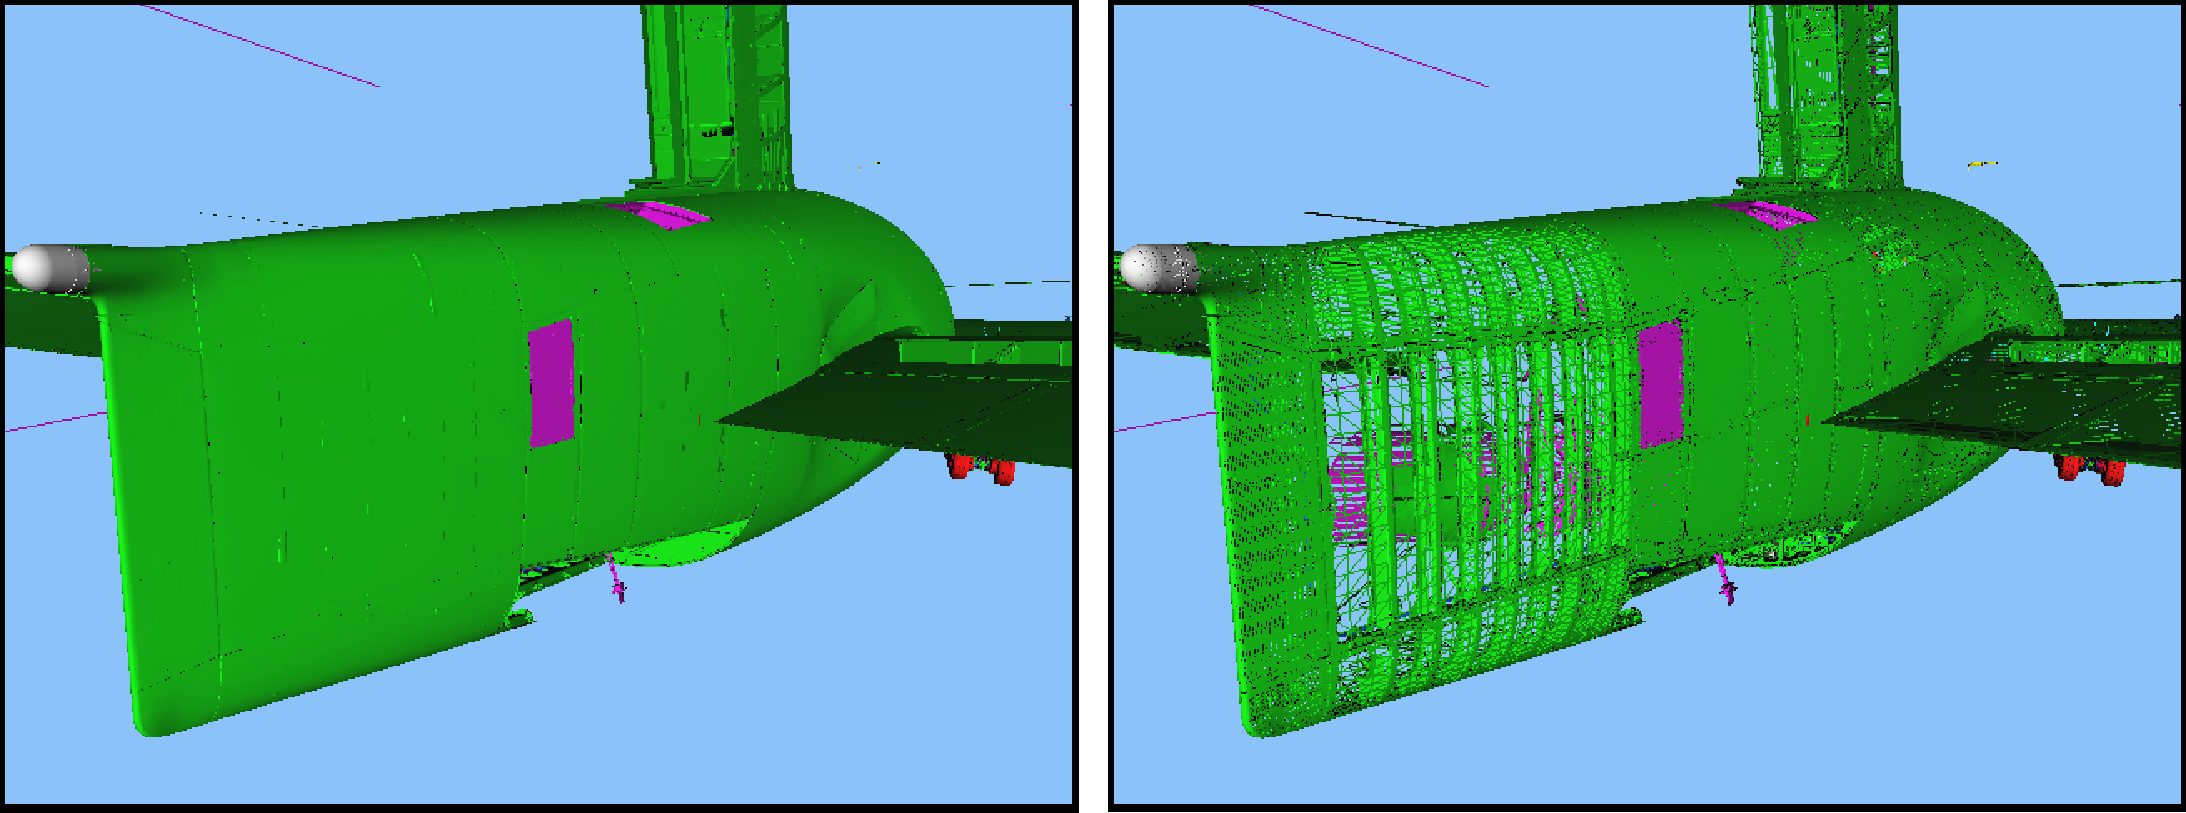
\includegraphics[scale=0.40]{images/pos1.pdf}
\captionof{figure}{\label{fig:eval:pos1}Kameraposition 1 \textit{(Heck außen, 3.352.475 sichtbare Dreiecke)}}
\end{Bild}

\begin{Bild}
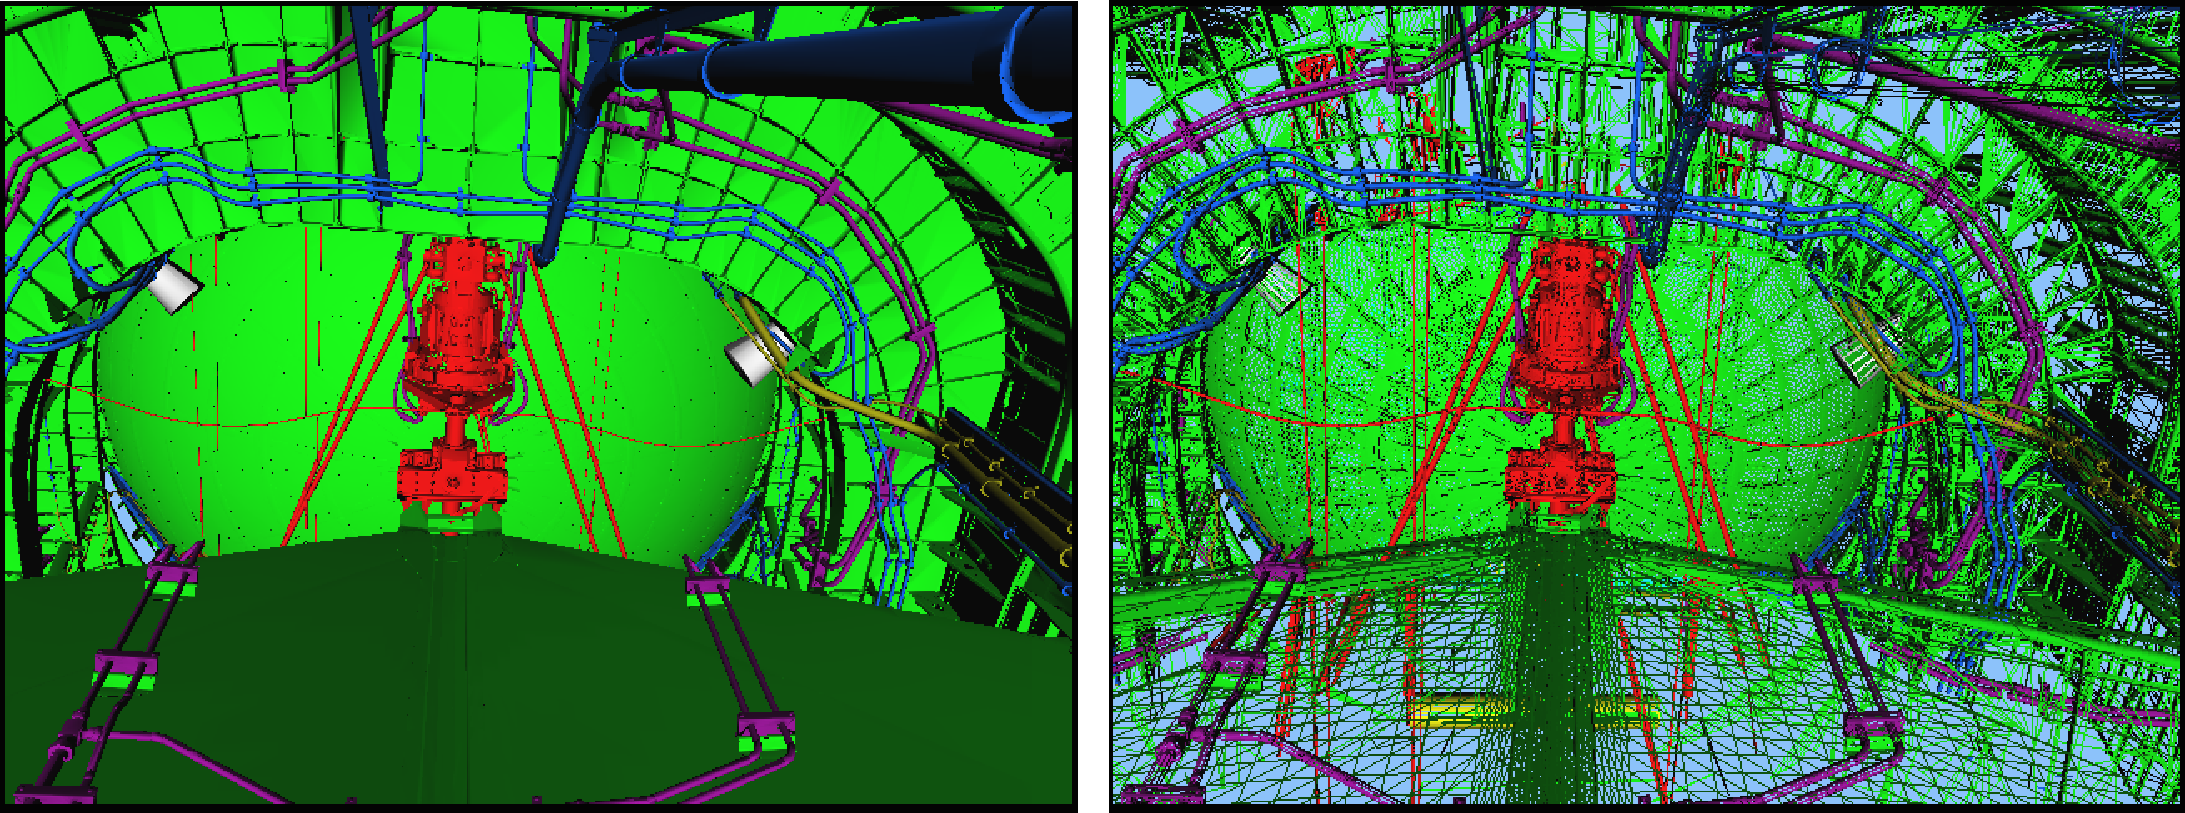
\includegraphics[scale=0.40]{images/pos2.pdf}
\captionof{figure}{\label{fig:eval:pos2}Kameraposition 2 \textit{(Heck innen, 2.045.104 sichtbare Dreiecke)}}
\end{Bild}

\begin{Bild}
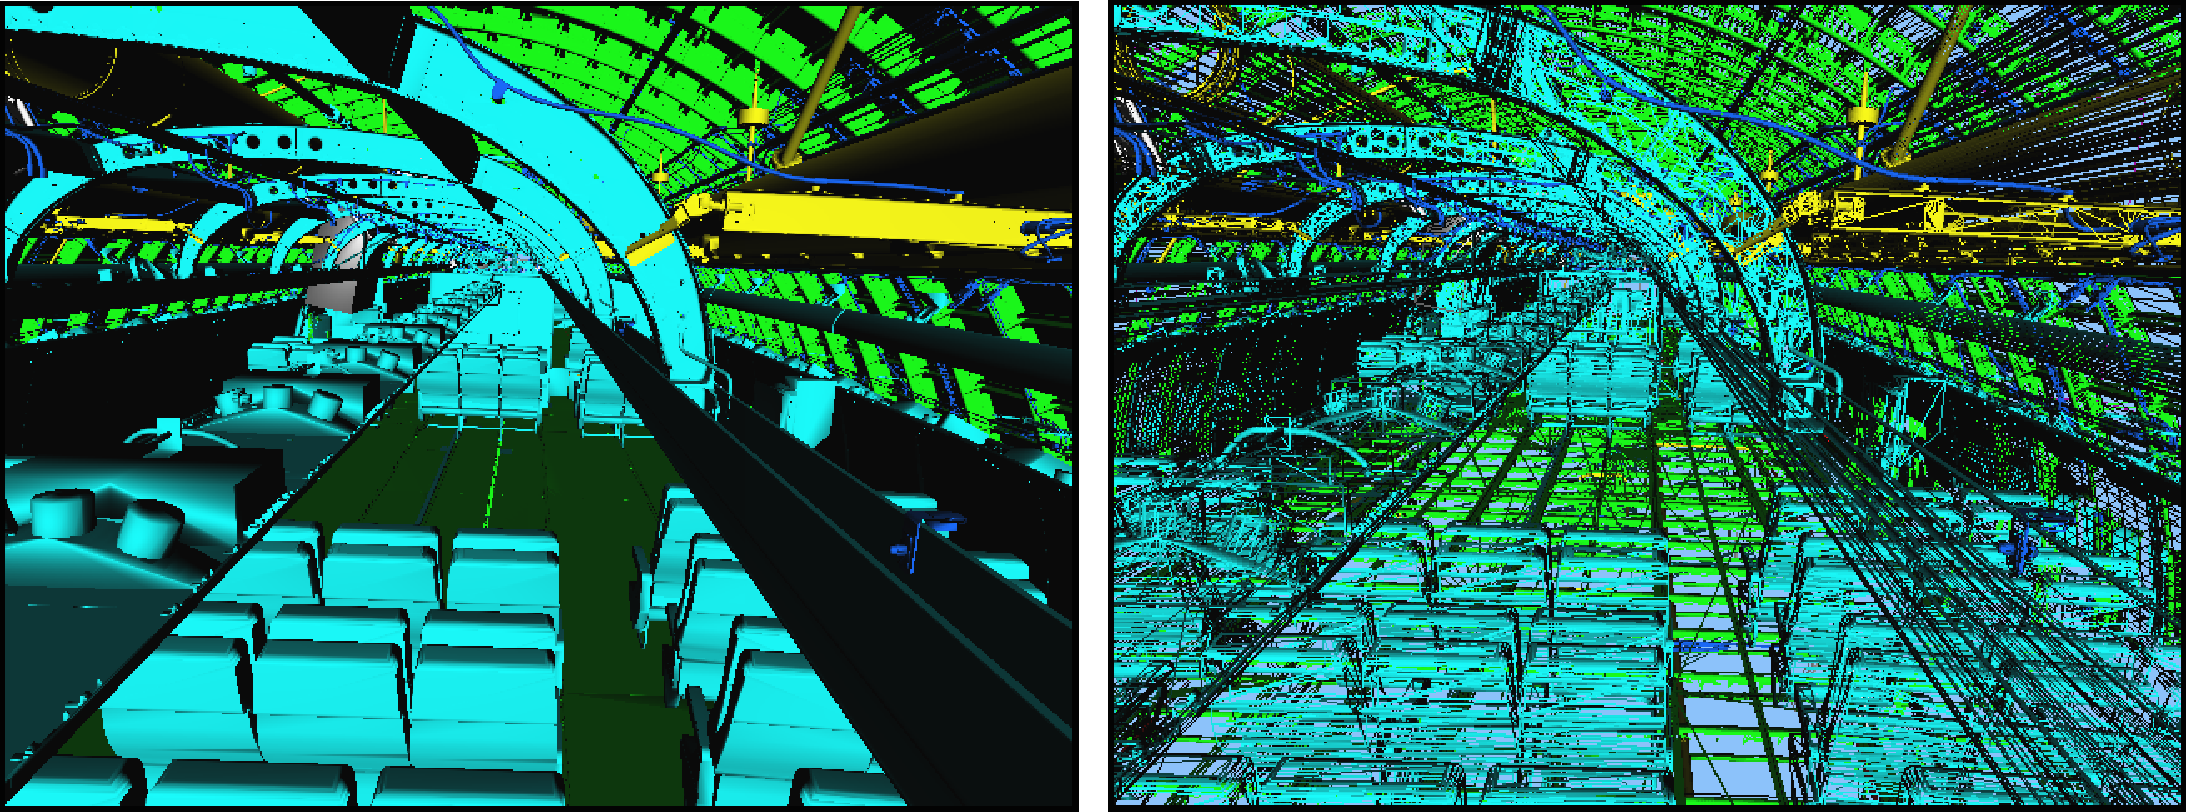
\includegraphics[scale=0.40]{images/pos3.pdf}
\captionof{figure}{\label{fig:eval:pos3}Kameraposition 3 \textit{(Passagierbereich, 3.749.977 sichtbare Dreiecke)}}
\end{Bild}

\begin{Bild}
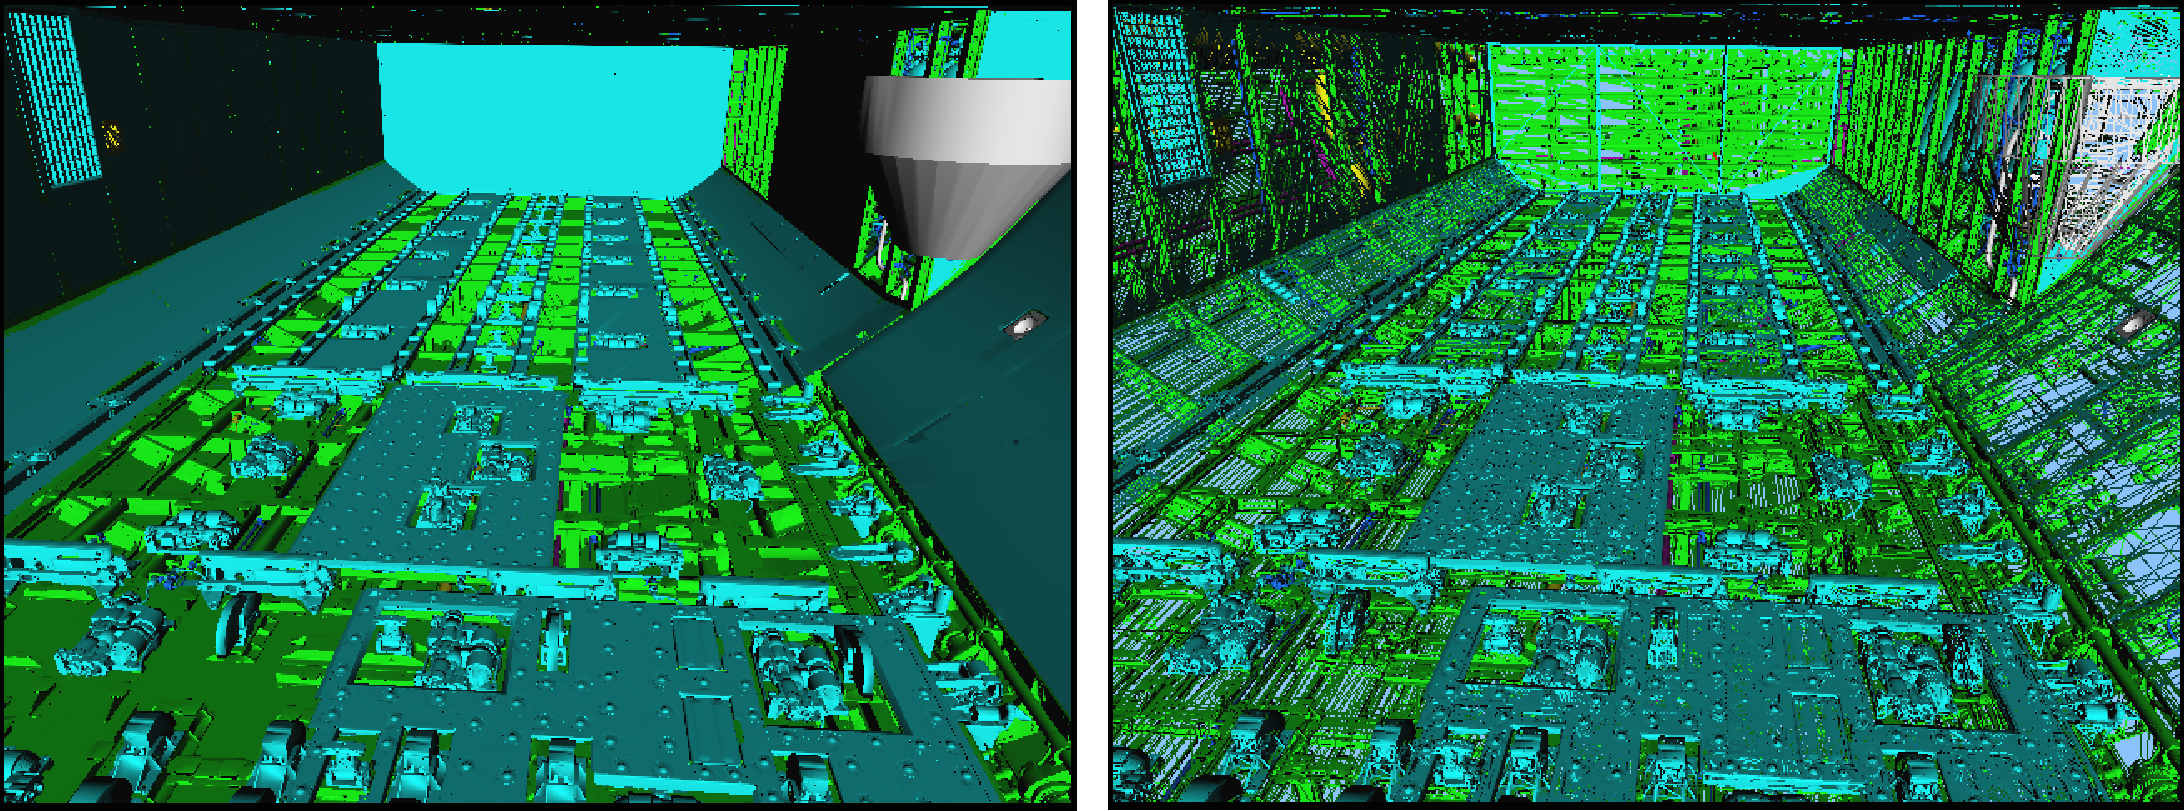
\includegraphics[scale=0.40]{images/pos4.pdf}
\captionof{figure}{\label{fig:eval:pos4}Kameraposition 4 \textit{(Stauraum, 8.381.277 sichtbare Dreiecke)}}
\end{Bild}

\begin{Bild}
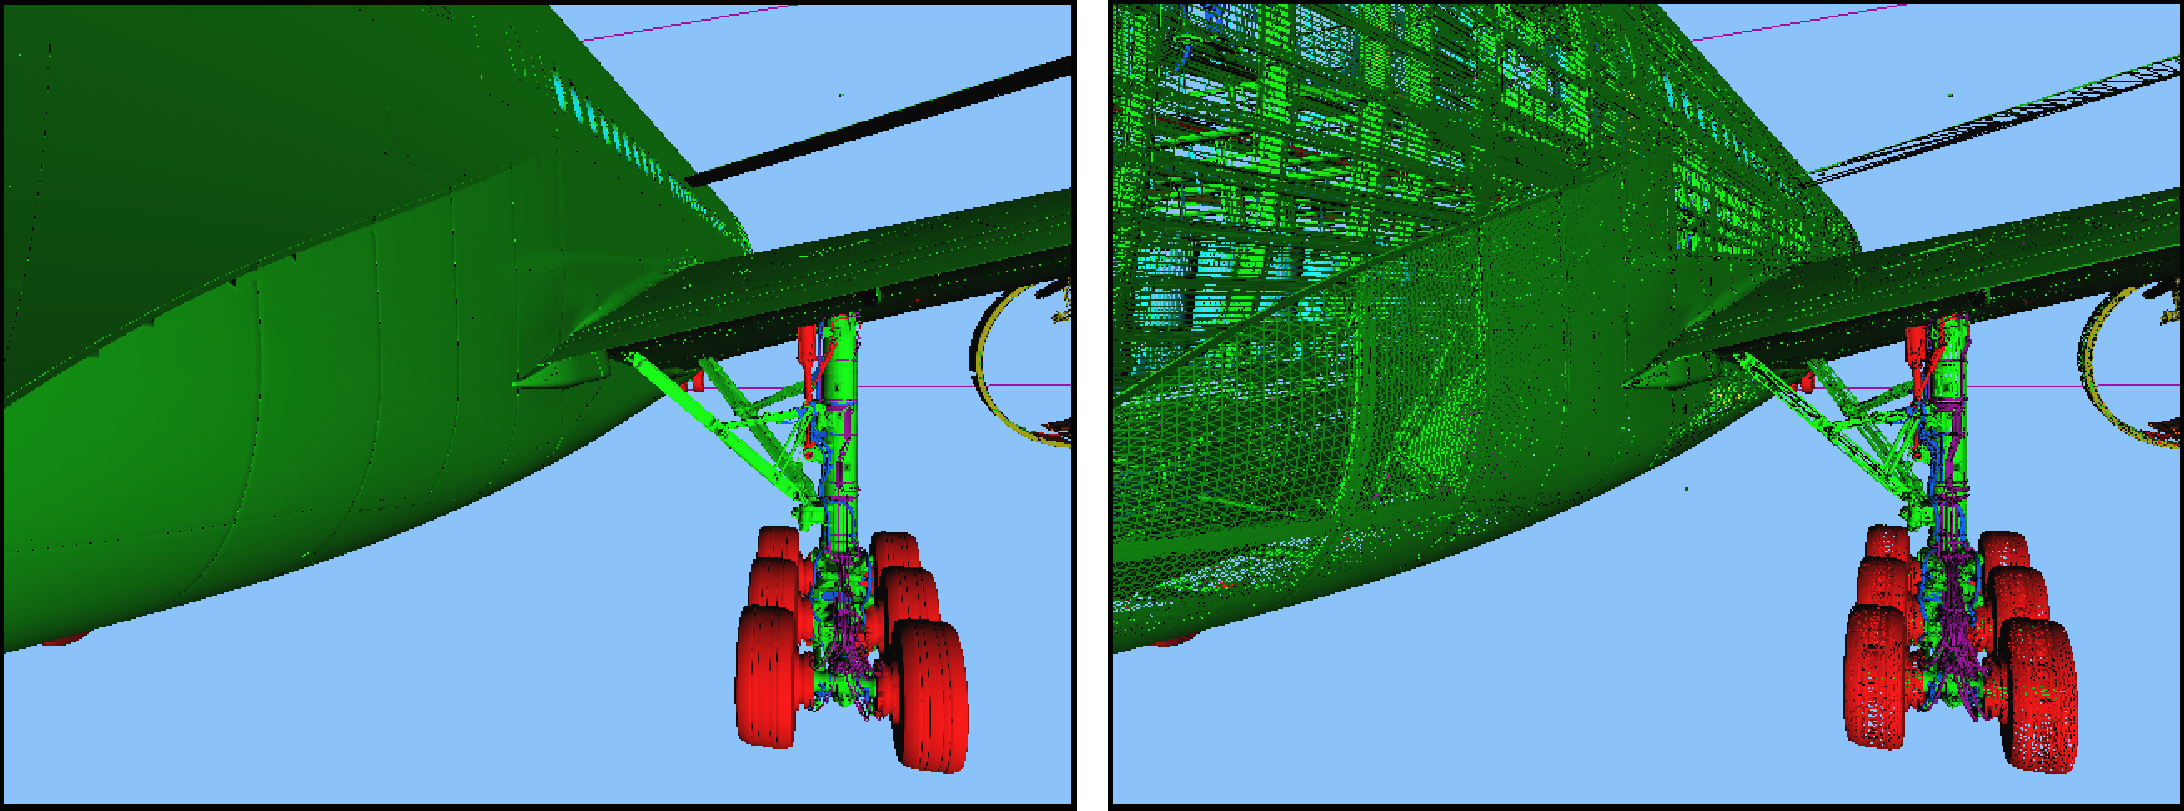
\includegraphics[scale=0.40]{images/pos5.pdf}
\captionof{figure}{\label{fig:eval:pos5}Kameraposition 5 \textit{(Fahrwerk/Flügel, 5.776.159 sichtbare Dreiecke)}}
\end{Bild}

\begin{Bild}
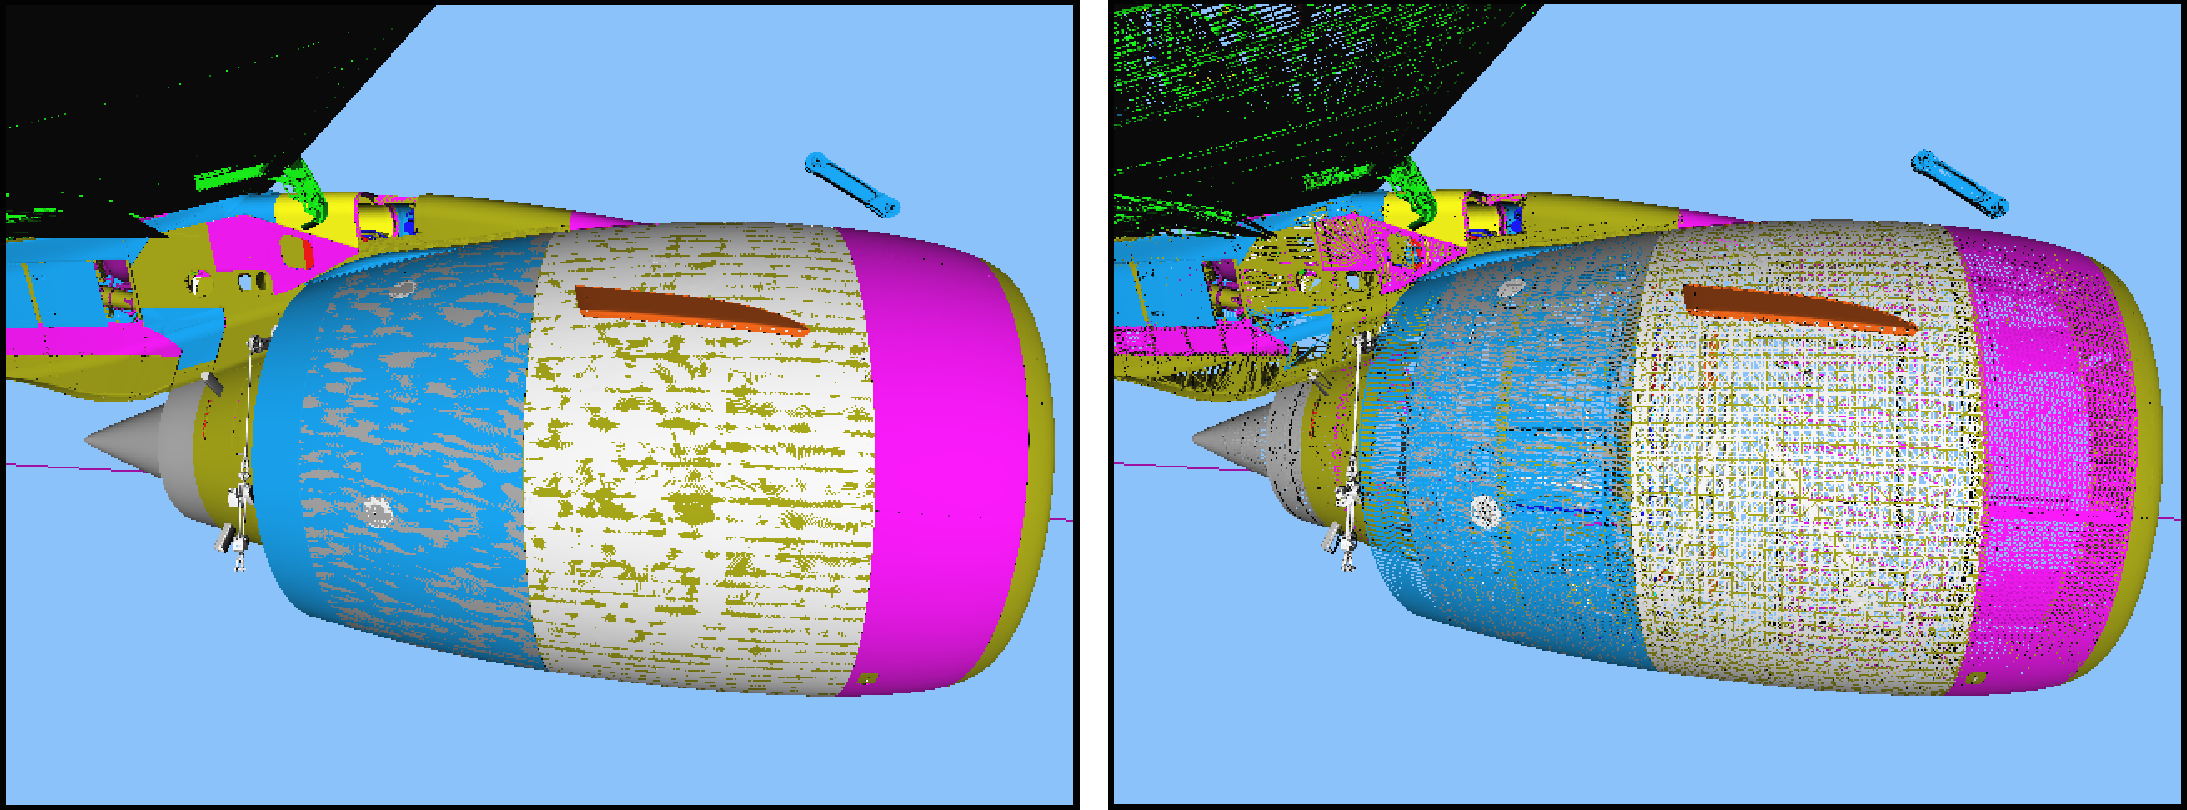
\includegraphics[scale=0.40]{images/pos6.pdf}
\captionof{figure}{\label{fig:eval:pos6}Kameraposition 6 \textit{(Turbine, 3.381.998 sichtbare Dreiecke)}}
\end{Bild}

\begin{Bild}
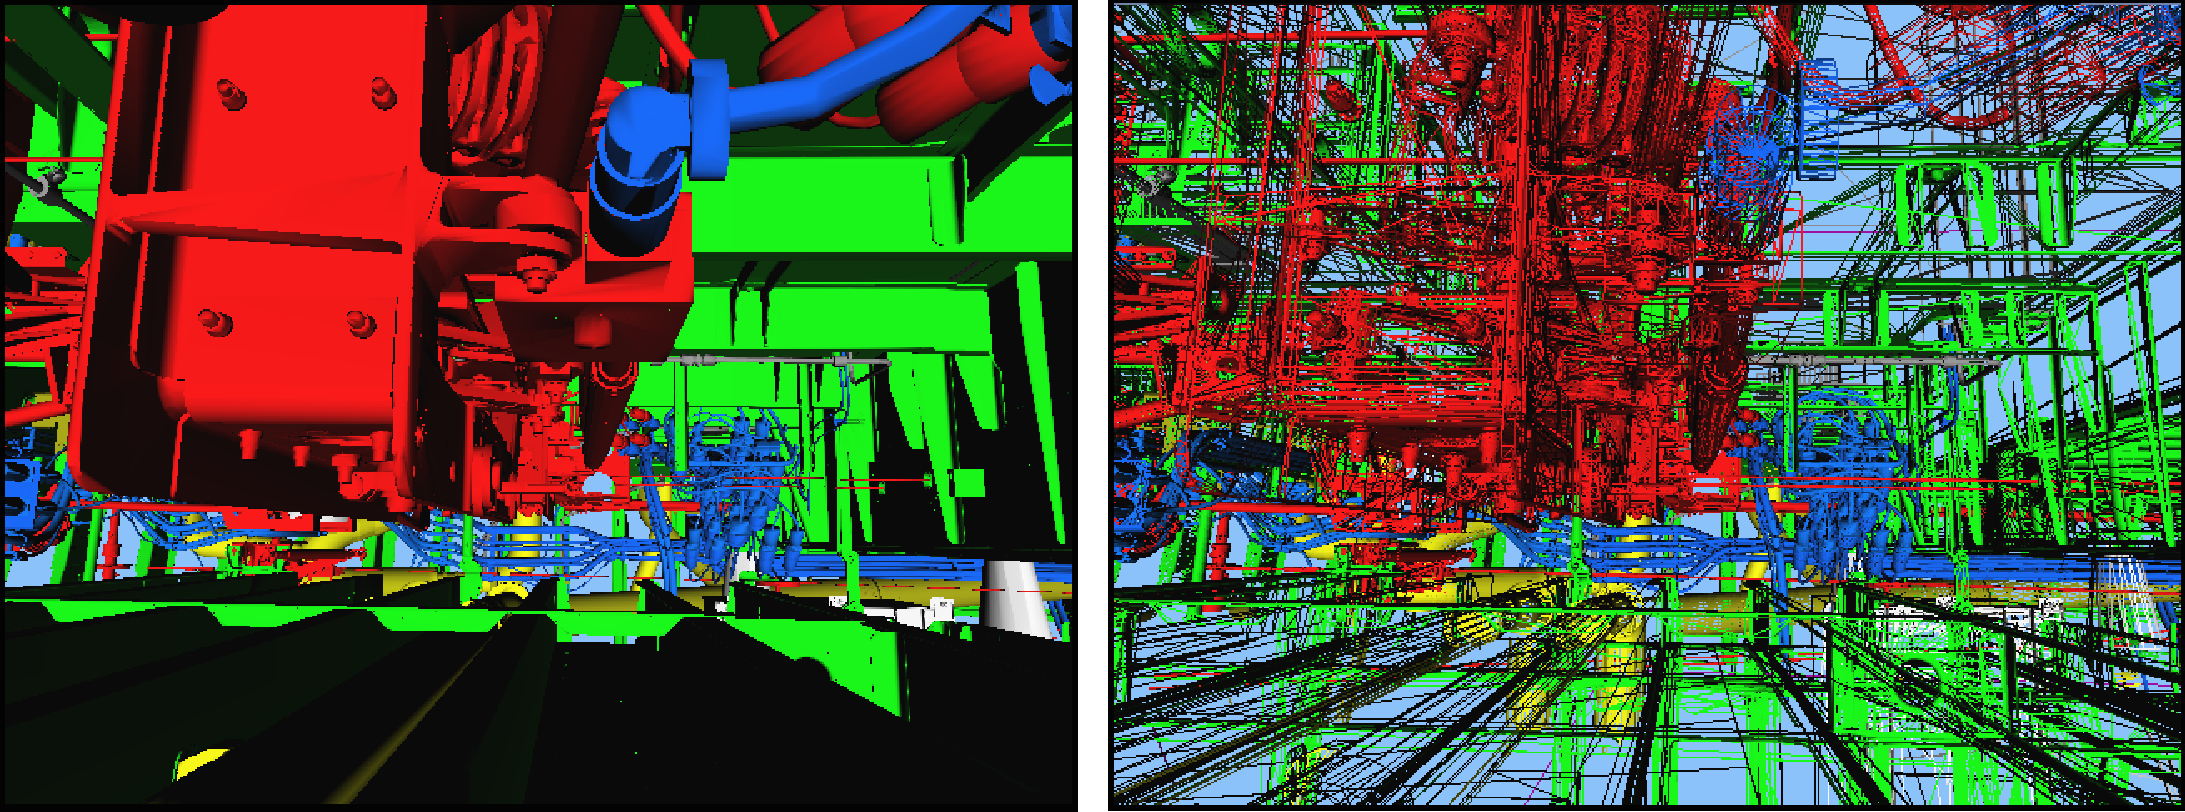
\includegraphics[scale=0.40]{images/pos7.pdf}
\captionof{figure}{\label{fig:eval:pos7}Kameraposition 7 \textit{(Nase innen, 1.481.706 sichtbare Dreiecke)}}
\end{Bild}

\begin{Bild}
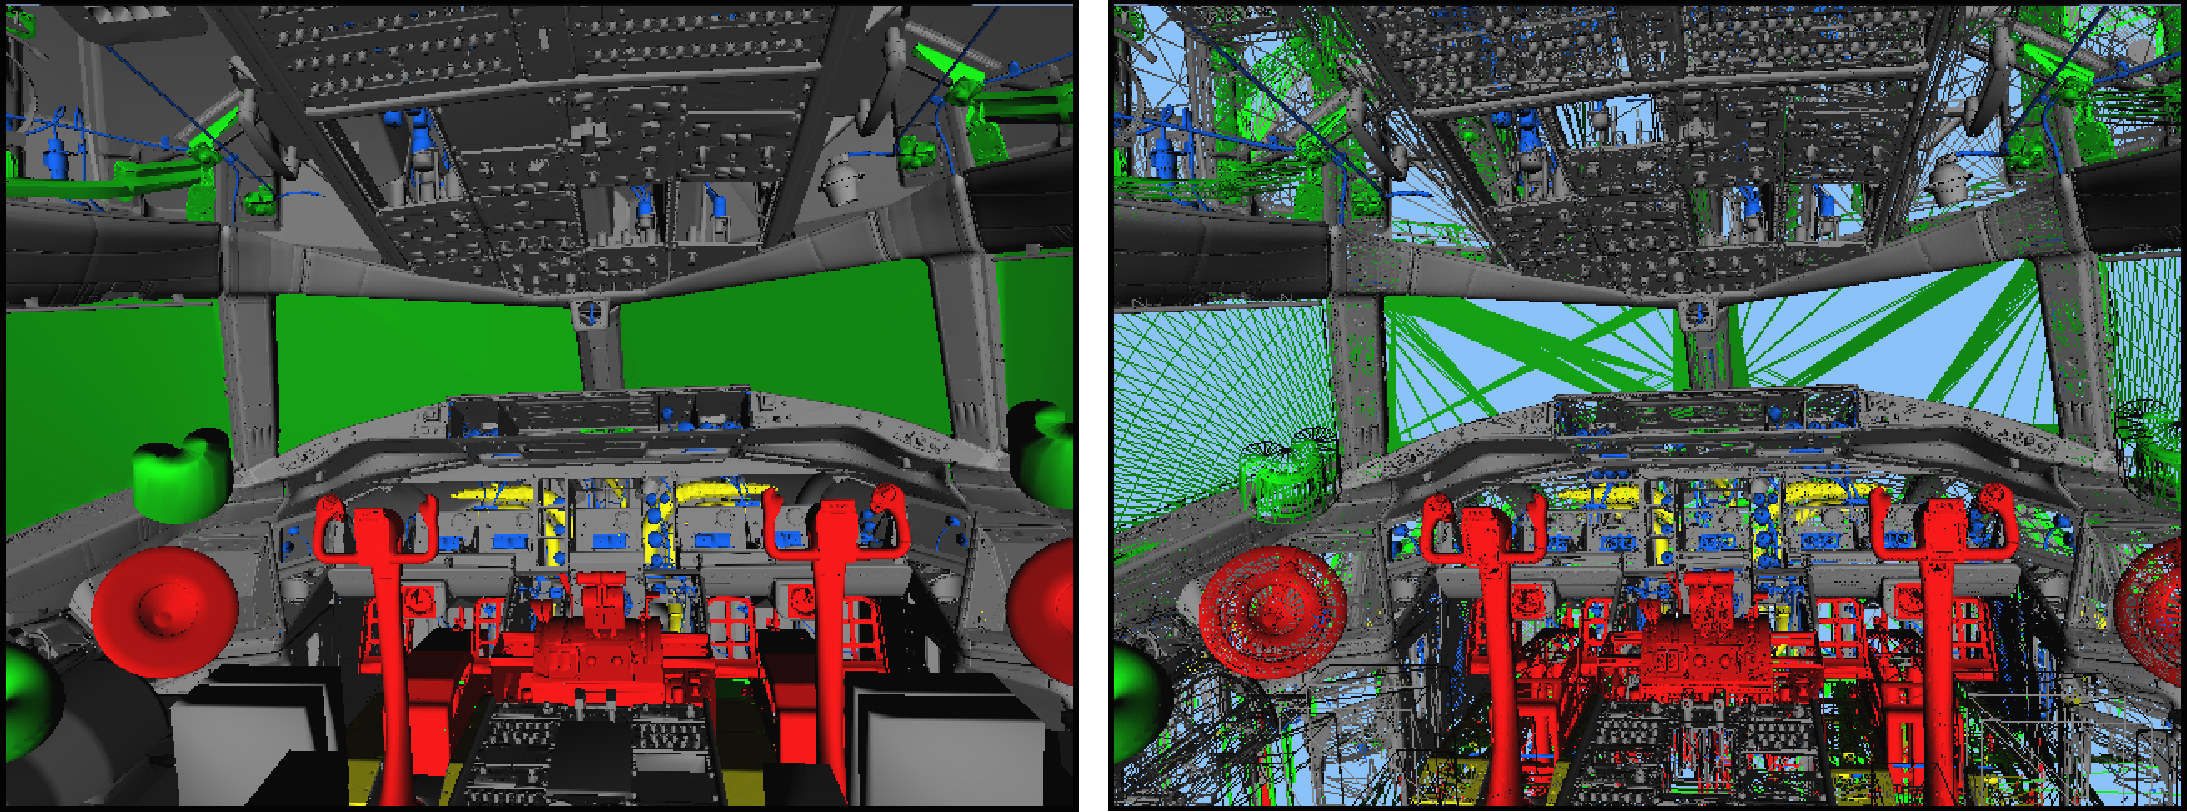
\includegraphics[scale=0.40]{images/pos8.pdf}
\captionof{figure}{\label{fig:eval:pos8}Kameraposition 8 \textit{(Cockpit, 4.558.623 sichtbare Dreiecke)}}
\end{Bild}

\begin{Bild}
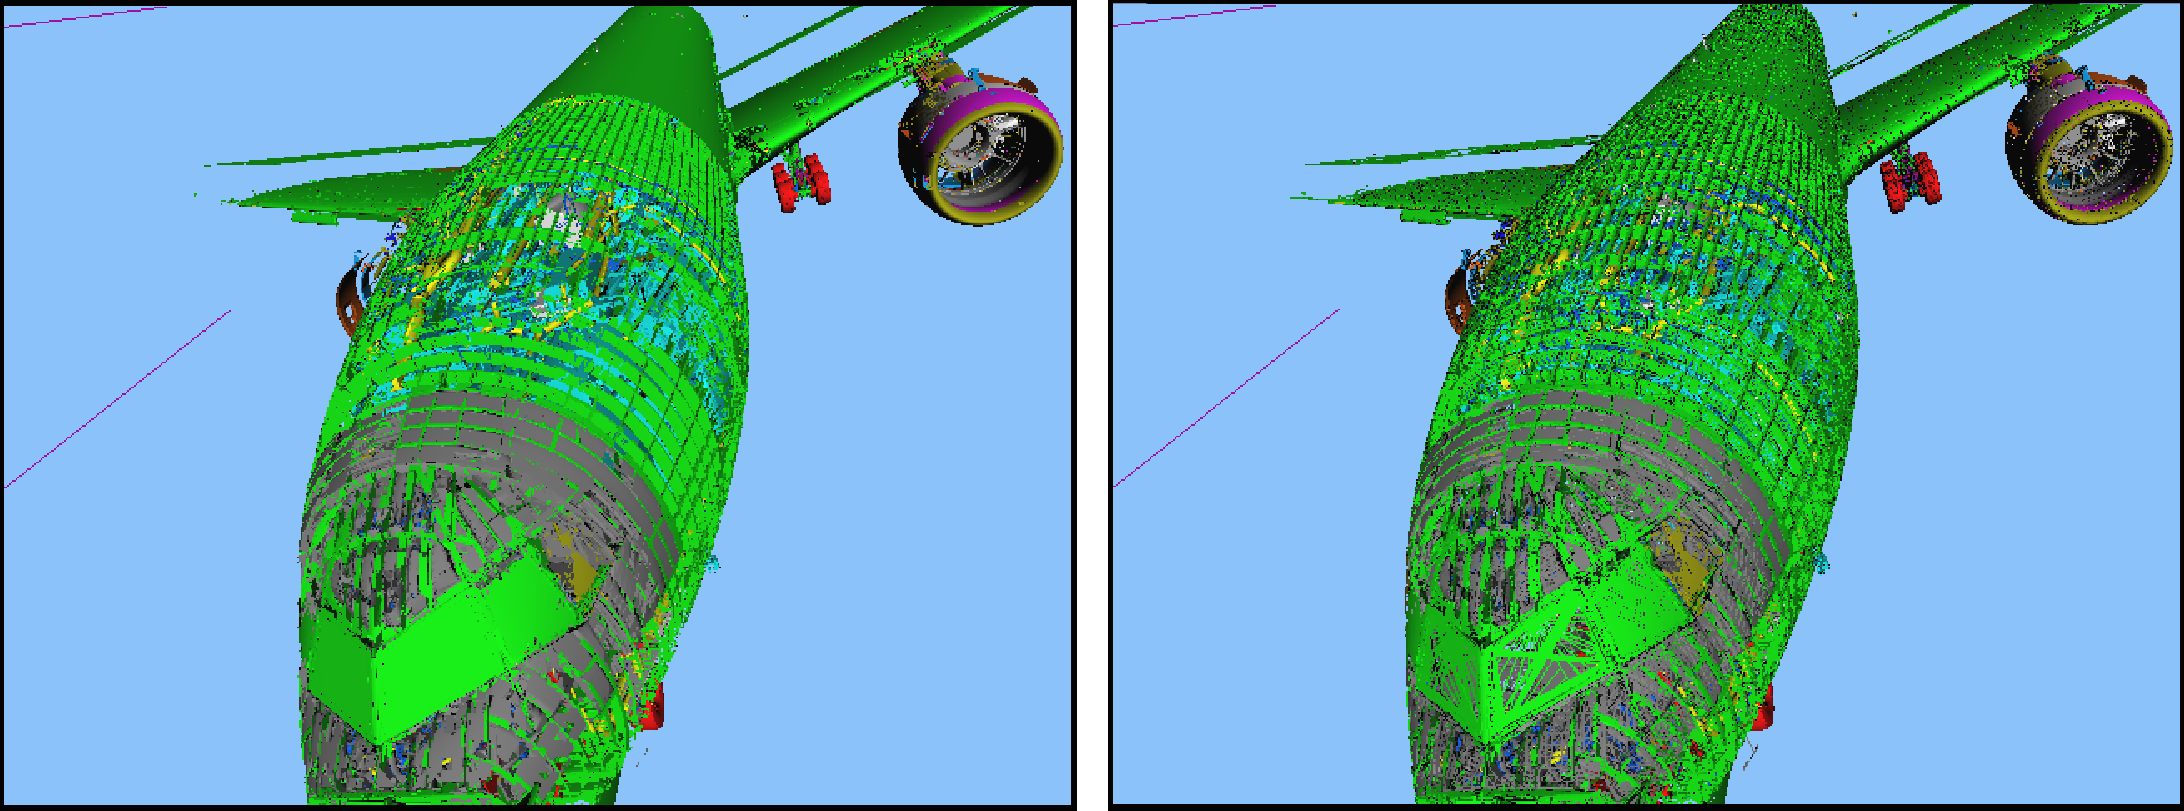
\includegraphics[scale=0.40]{images/pos9.pdf}
\captionof{figure}{\label{fig:eval:pos9}Kameraposition 9 \textit{(Nase außen, 7.439.695 sichtbare Dreiecke)}}
\end{Bild}

\begin{Bild}
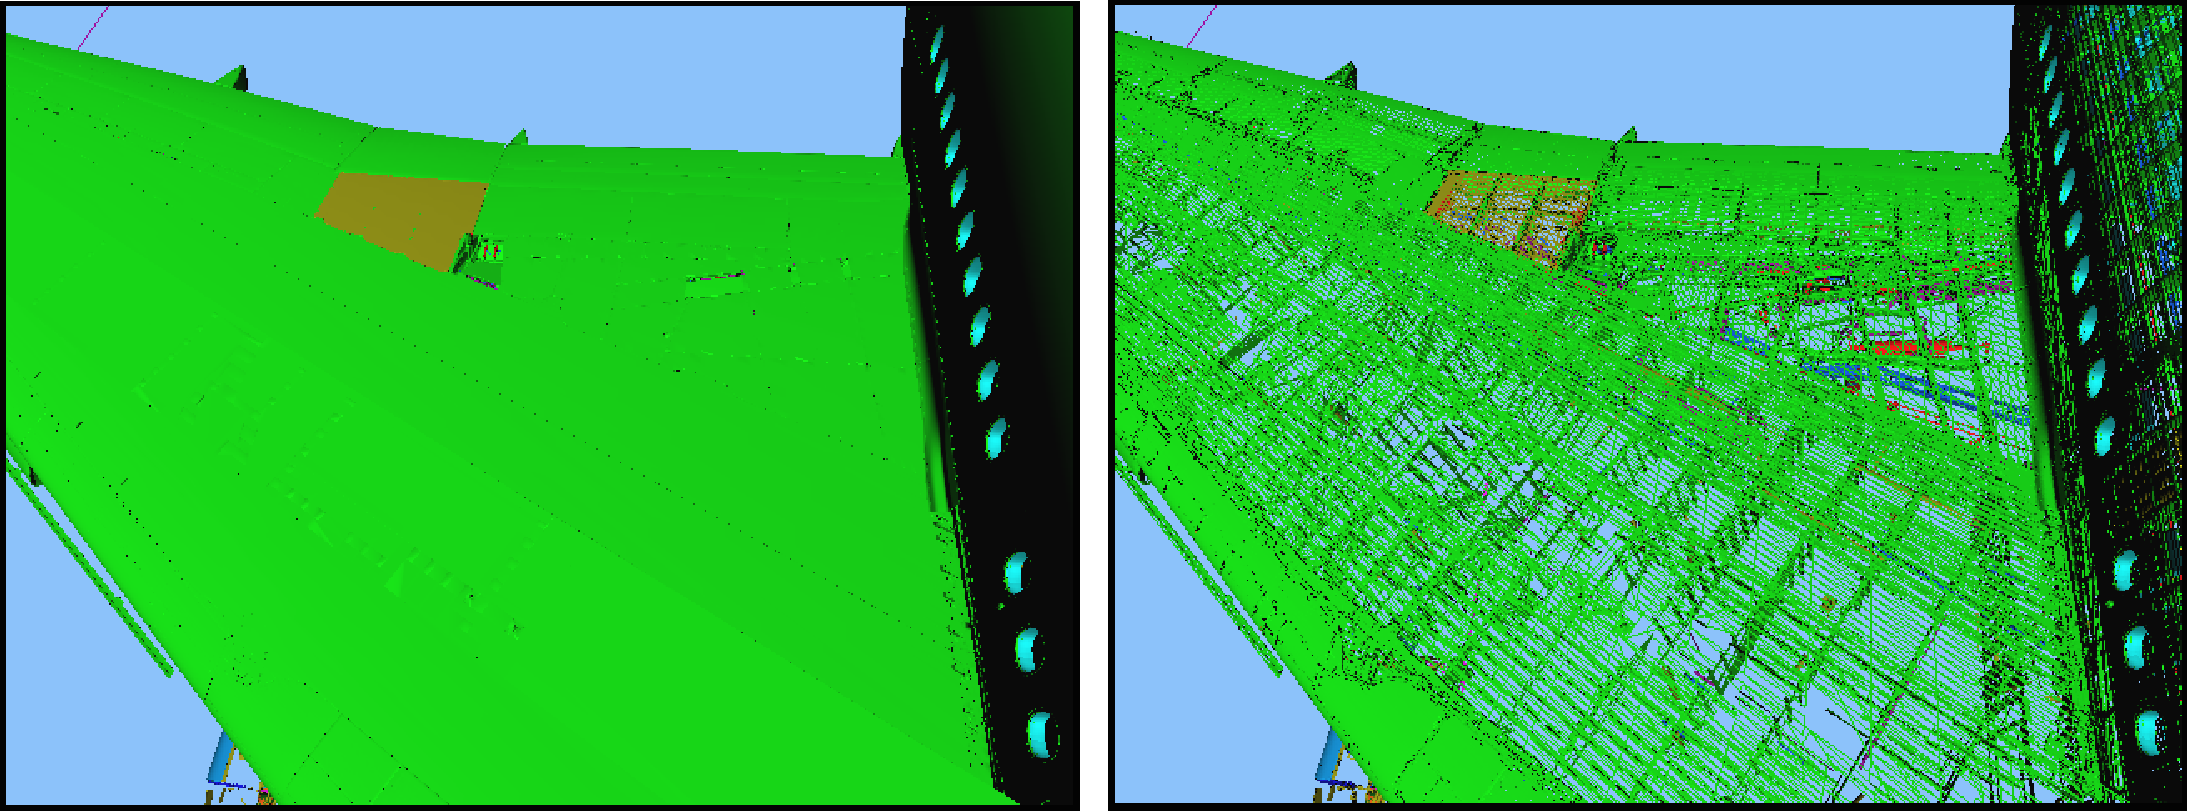
\includegraphics[scale=0.40]{images/pos10.pdf}
\captionof{figure}{\label{fig:eval:pos10}Kameraposition 10 \textit{(Flügel-Rumpf Bereich, 4.066.296 sichtbare Dreiecke)}}
\end{Bild}

\begin{Bild}
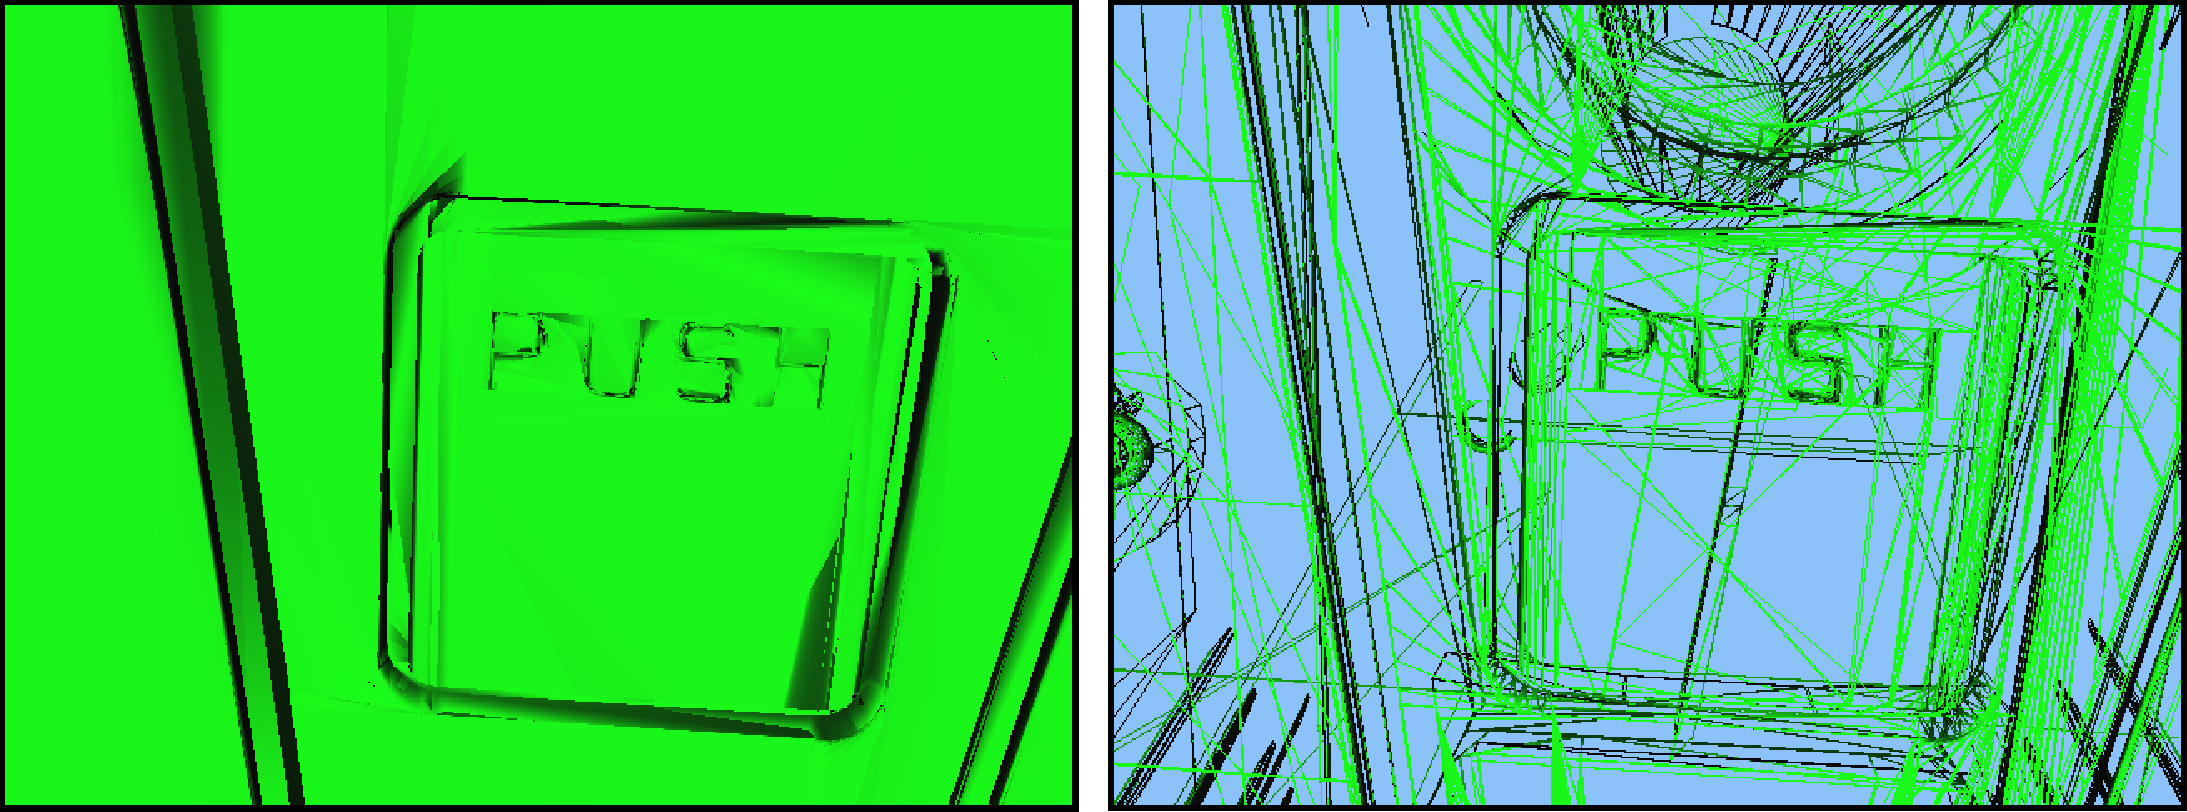
\includegraphics[scale=0.40]{images/button.pdf}
\captionof{figure}{\label{fig:eval:button}Türknopf \textit{(Bug)}}
\end{Bild}

\begin{Bild}
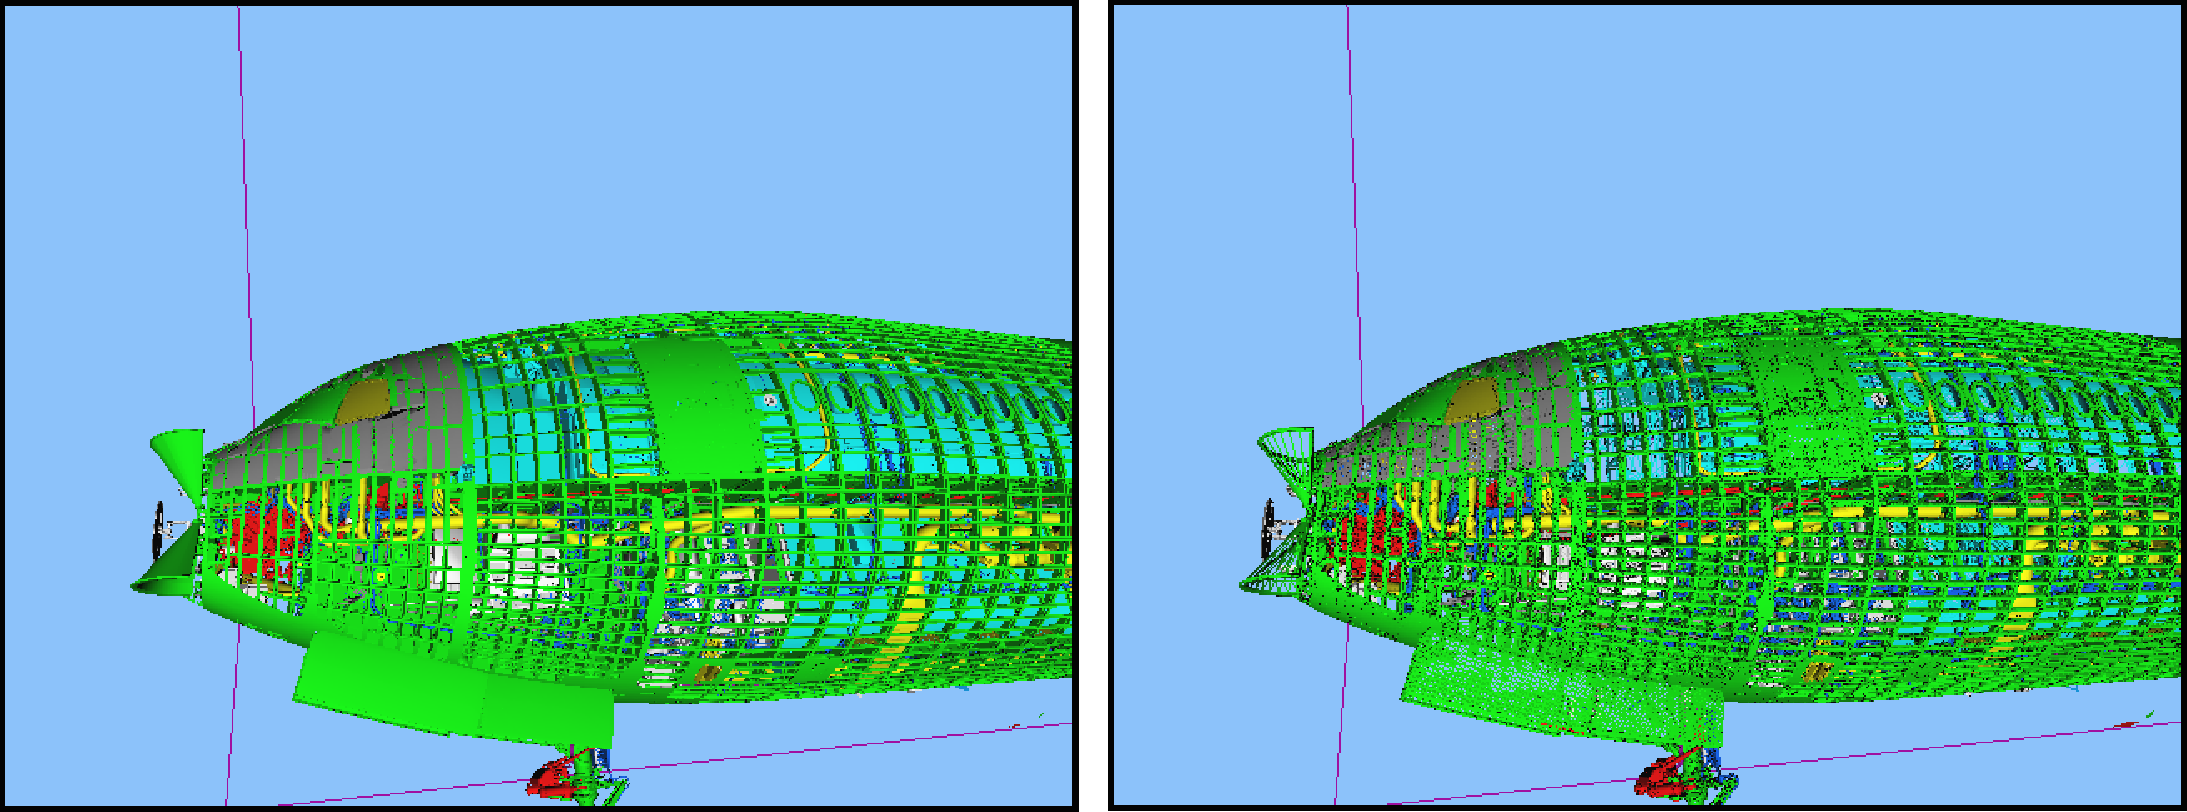
\includegraphics[scale=0.40]{images/profil_bug.pdf}
\captionof{figure}{\label{fig:eval:prof_bug}Profil \textit{(Bug)}}
\end{Bild}

\begin{Bild}
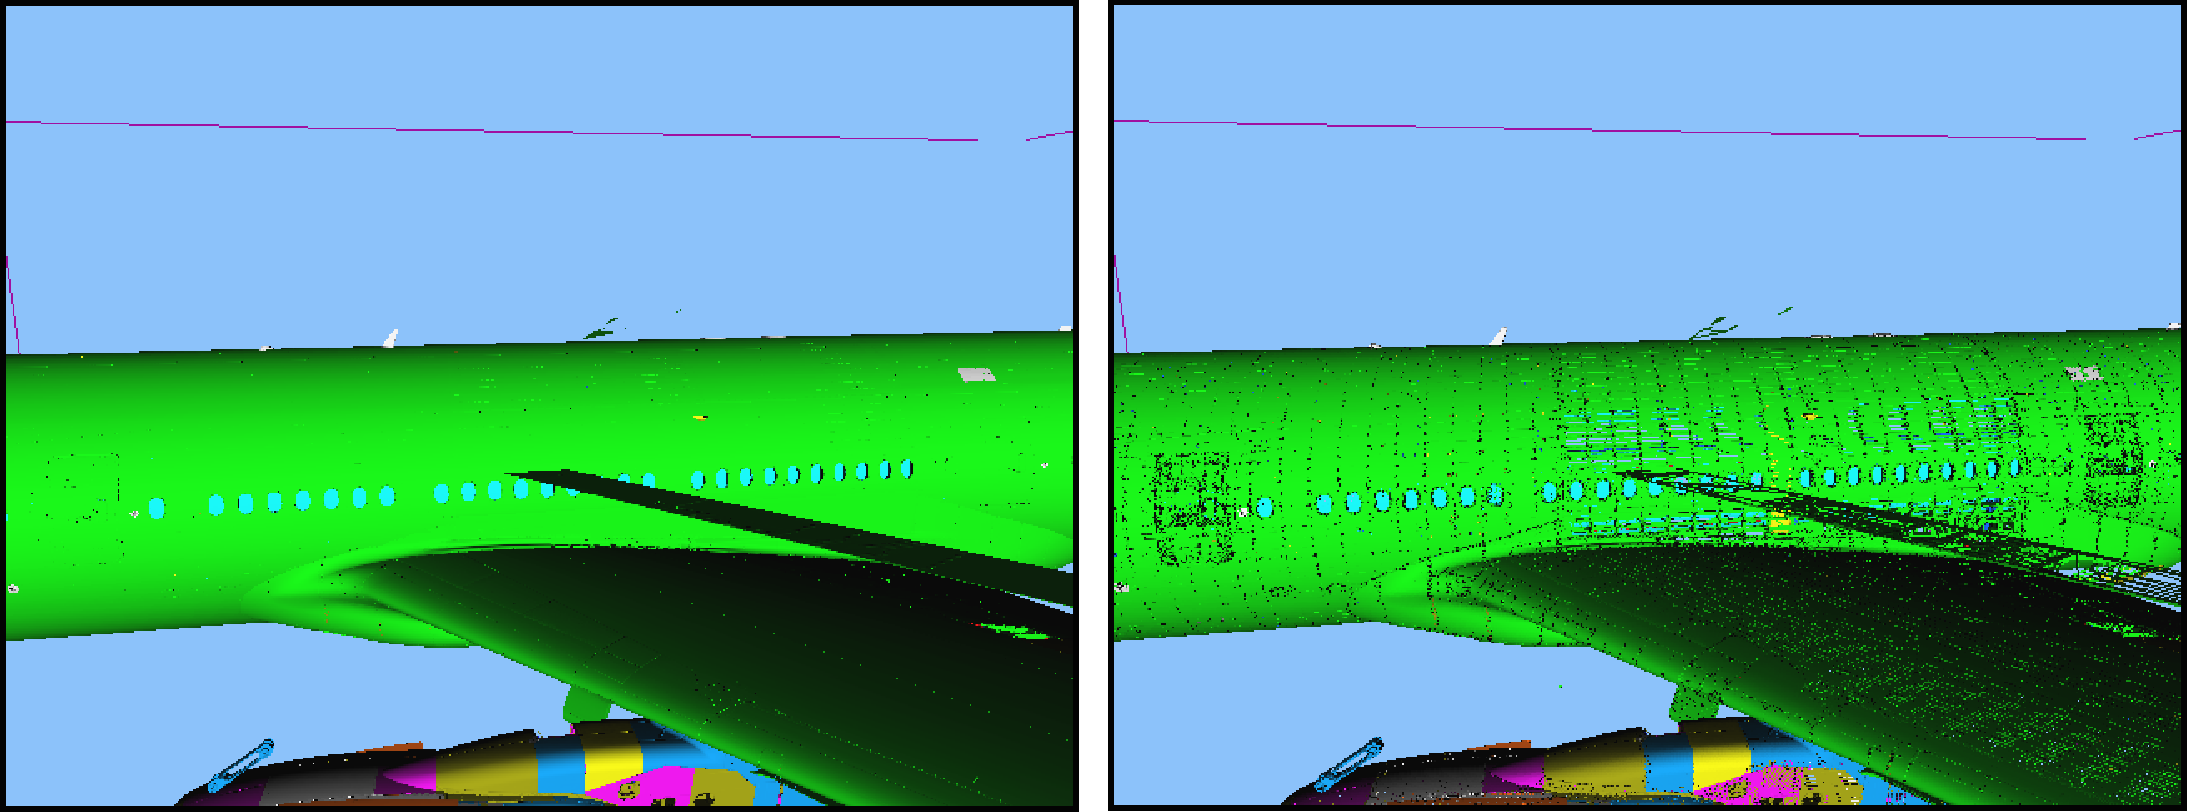
\includegraphics[scale=0.40]{images/profil_heck.pdf}
\captionof{figure}{\label{fig:eval:prof_heck}Profil \textit{(Heck)}}
\end{Bild}

\begin{Bild}
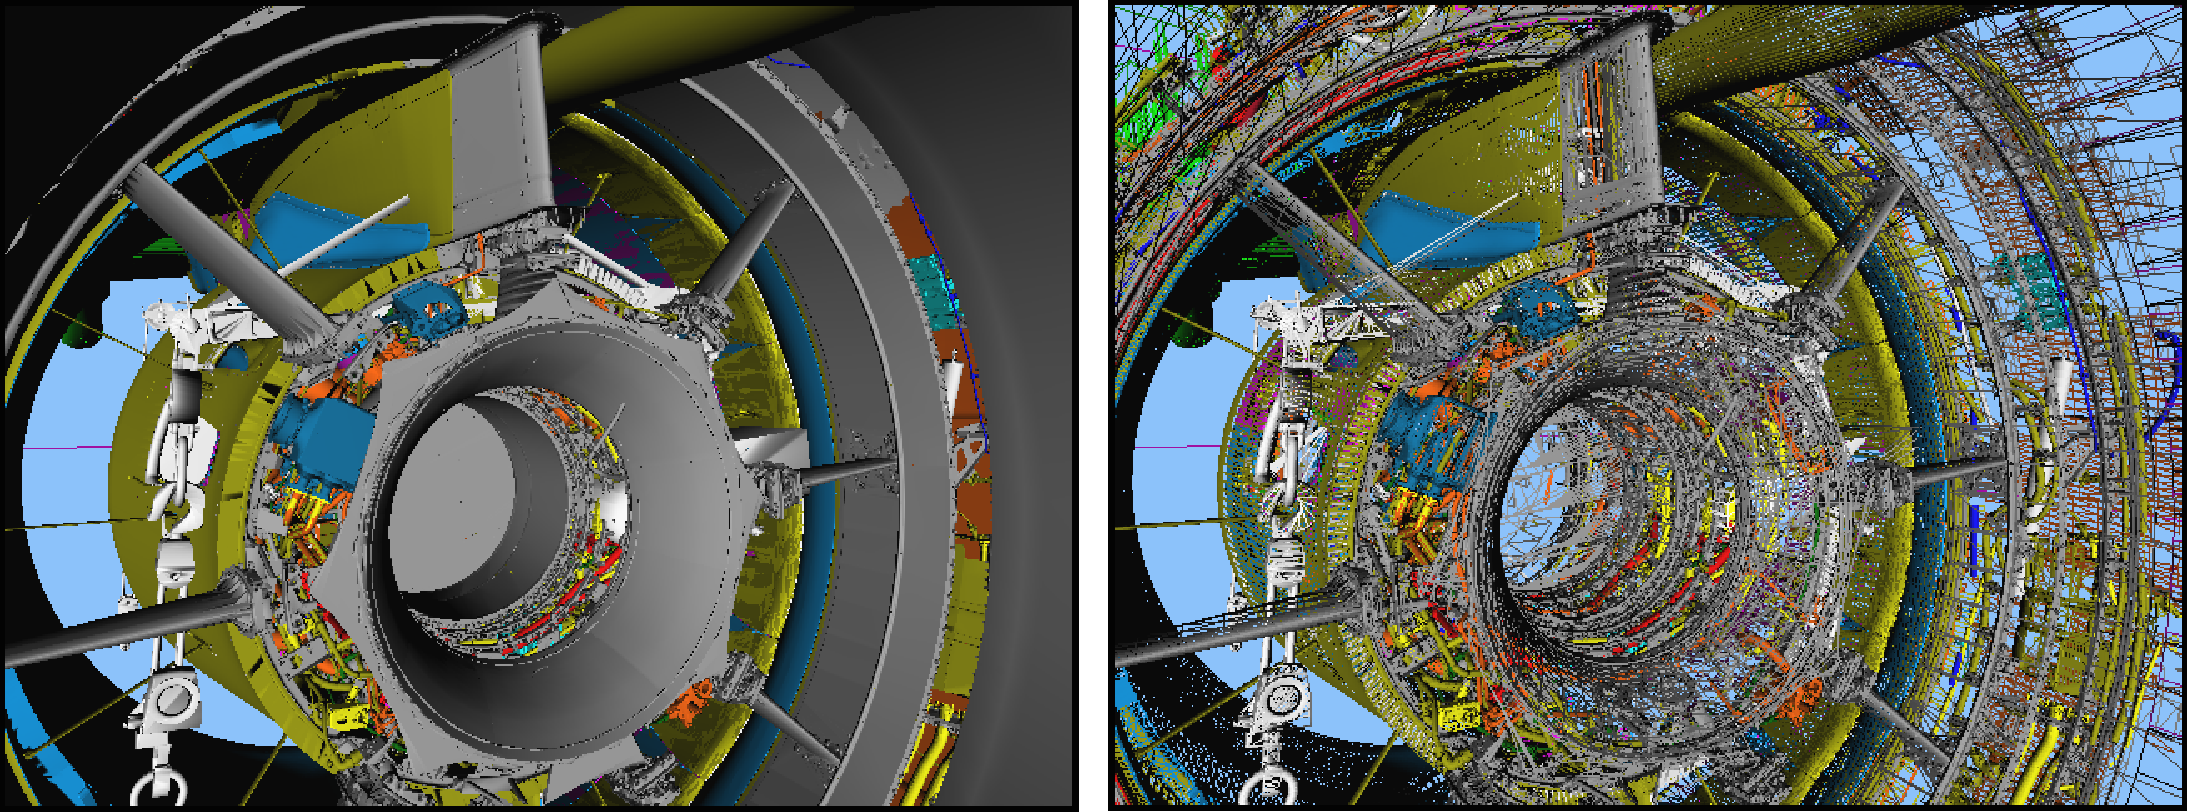
\includegraphics[scale=0.40]{images/turbine_innen.pdf}
\captionof{figure}{\label{fig:eval:turbine_innen}Triebwerk 1}
\end{Bild}

\begin{Bild}
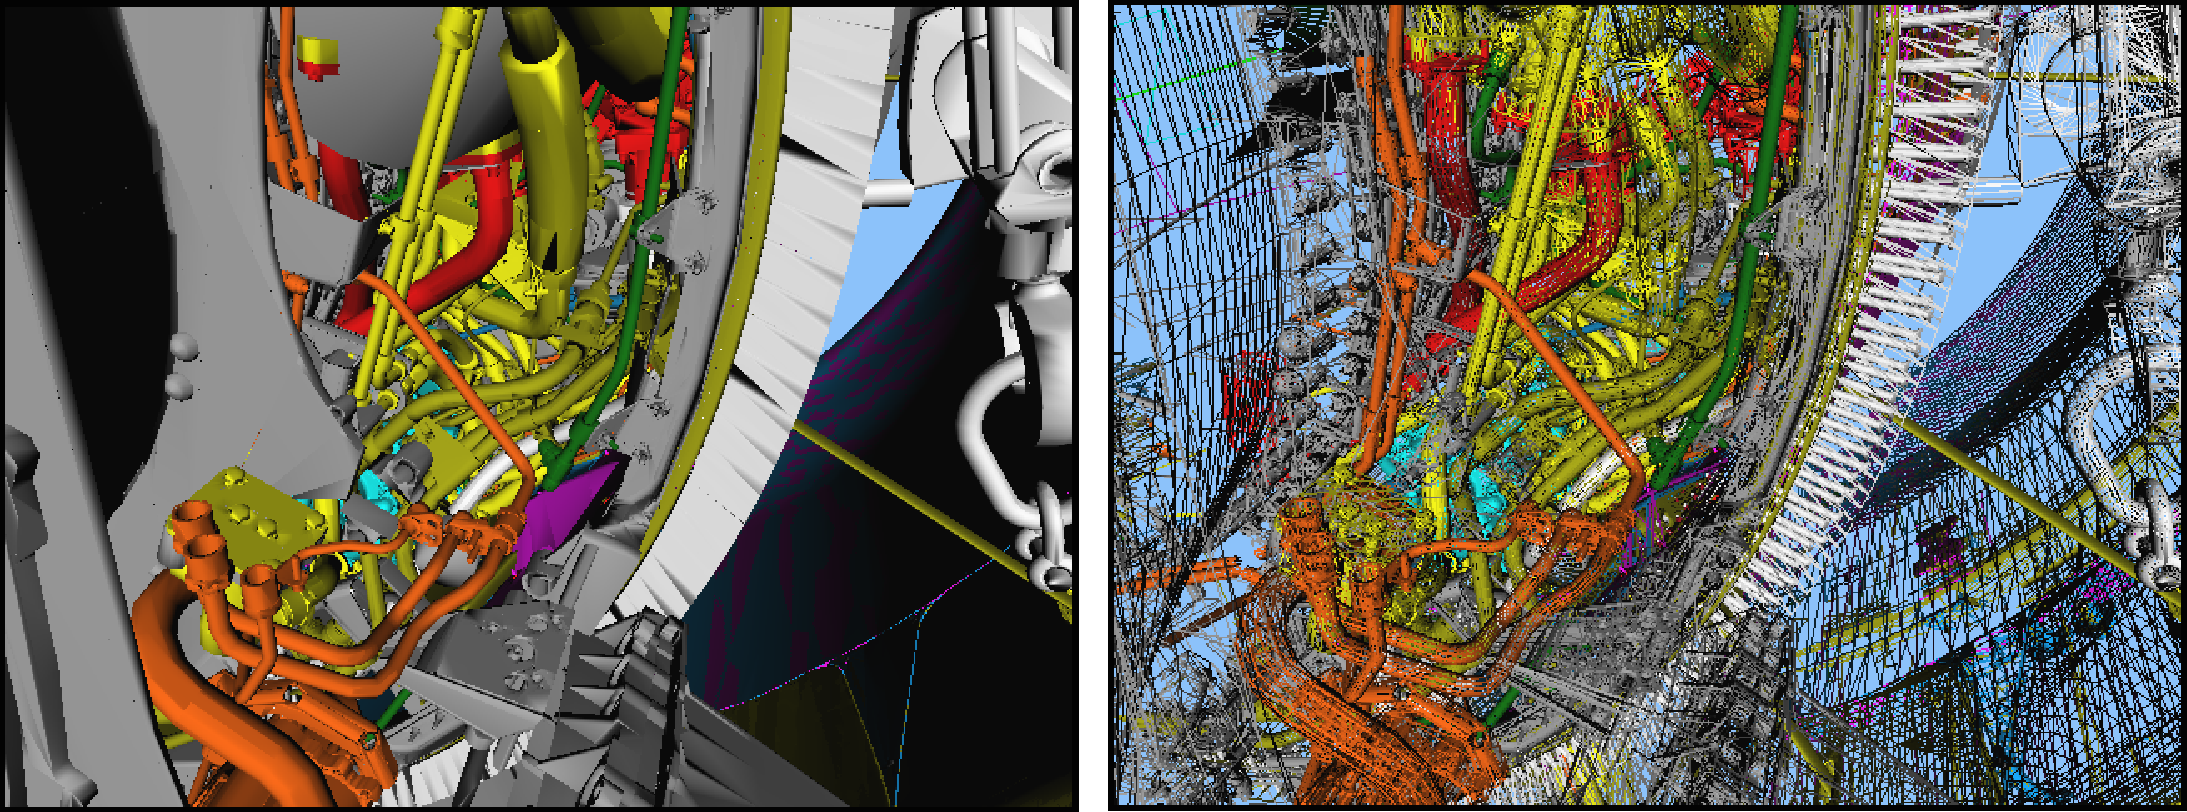
\includegraphics[scale=0.40]{images/turbine_innen2.pdf}
\captionof{figure}{\label{fig:eval:turbine_innen2}Triebwerk 2}
\end{Bild}

\begin{Bild}
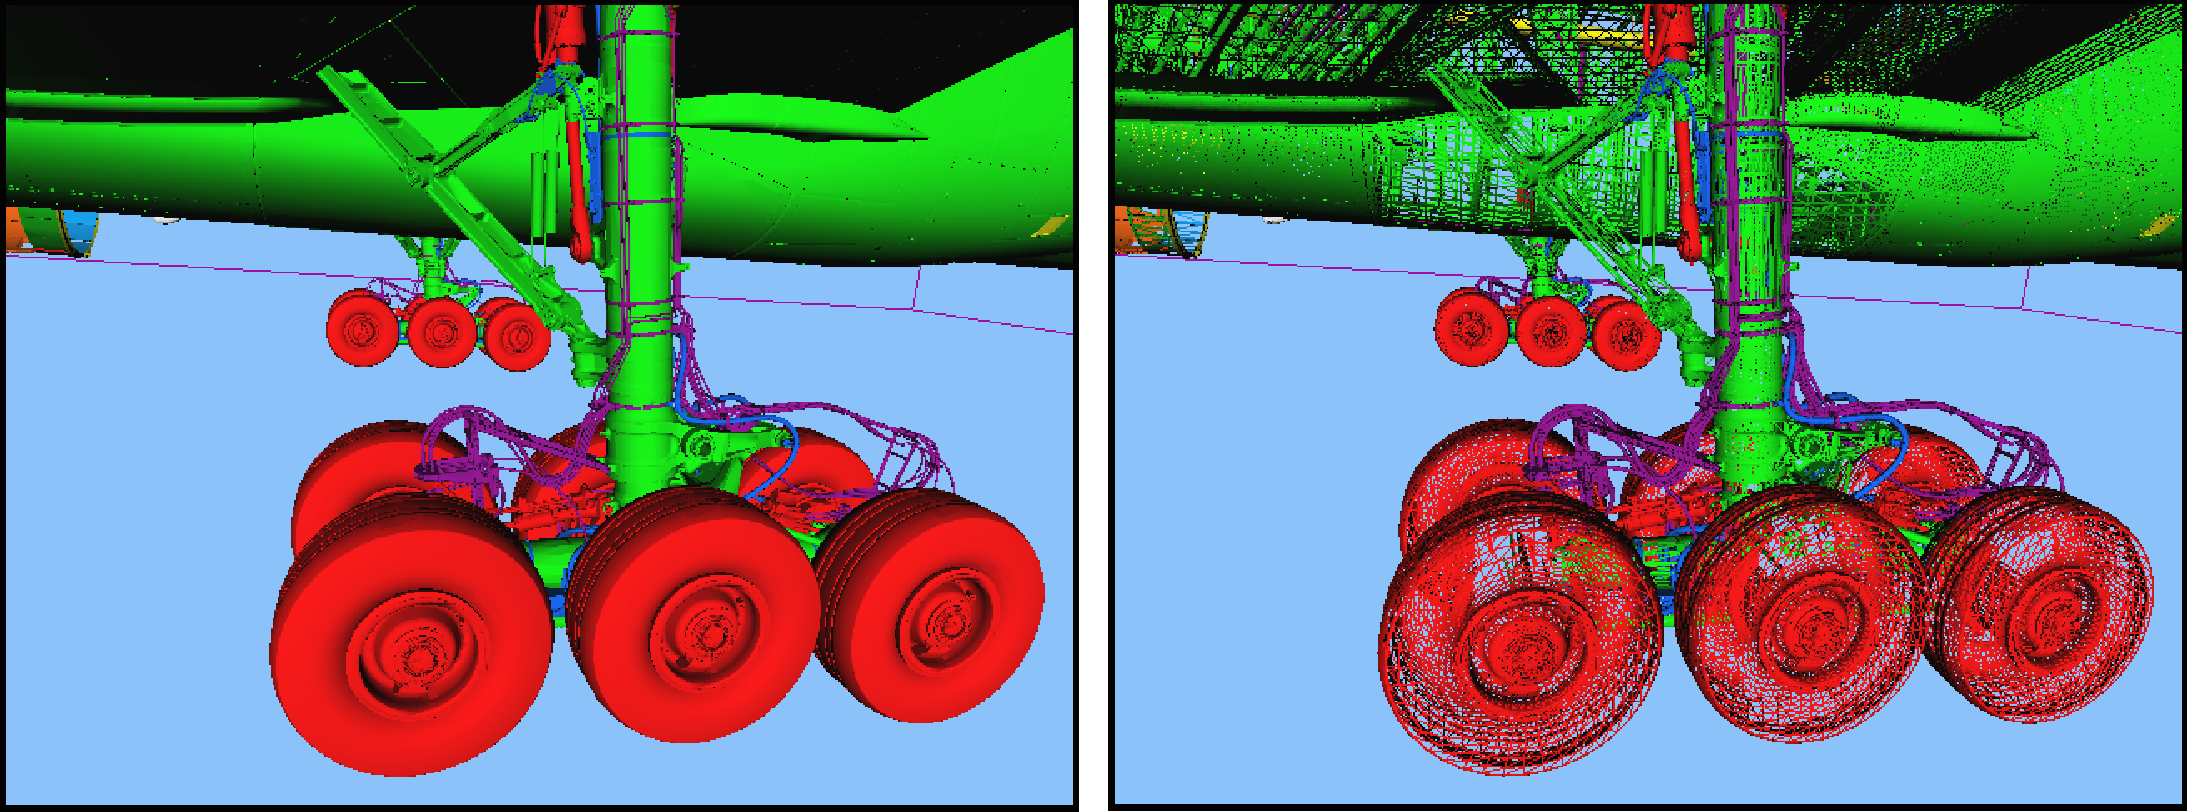
\includegraphics[scale=0.40]{images/fahrwerk.pdf}
\captionof{figure}{\label{fig:eval:fahrwerk}Fahrwerk \textit{(Heck)}}
\end{Bild}

%
% EOF
%
